% 2008 年福建卷理科第 18 题：四棱锥 P-ABCD，侧面 PAD⊥底面 ABCD，PA=PD=√2，
%   底面为直角梯形，BC∥AD，AB⊥AD，AD=2AB=2BC=2，O 为 AD 中点。
% 来源 PDF：gaokaomath-src/普通高考/2008/2008福建理.pdf
% SHA-256：516e8ac8e113868afa9bc4af4724c3b43f22a1f7fecc830a7f3400b8d973d452
% 原页：2008福建理.pdf 第 1 页（A3 三栏）第 3 栏，书页码 441。
% 重绘依据：与文科卷第 19 题同一幅图（同一几何体）：A 左、D 右、O 在 AD 上、B 左下、C 下中、
%   P 在 O 上方；P—A、P—B、P—C、P—D、A—B、B—C、C—D 实线，A—D（含 O）与 P—O 虚线。
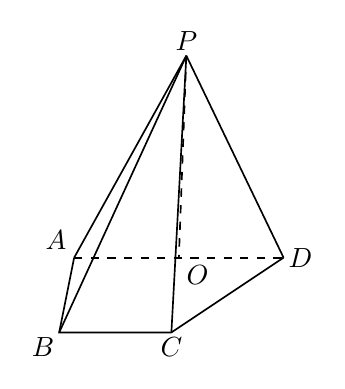
\begin{tikzpicture}[scale=0.95, semithick, every node/.style={inner sep=1.5pt}]
  \coordinate (P) at (1.70,4.00);
  \coordinate (A) at (0.20,1.30);
  \coordinate (D) at (3.00,1.30);
  \coordinate (O) at (1.60,1.30);
  \coordinate (B) at (0.00,0.30);
  \coordinate (C) at (1.50,0.30);

  \draw (P) -- (A);
  \draw (P) -- (B);
  \draw (P) -- (C);
  \draw (P) -- (D);
  \draw (A) -- (B) -- (C) -- (D);
  \draw[dashed] (A) -- (D);
  \draw[dashed] (P) -- (O);

  \node[above] at (P) {$P$};
  \node[above left=1pt] at (A) {$A$};
  \node[right] at (D) {$D$};
  \node[below right=1pt] at (O) {$O$};
  \node[below left] at (B) {$B$};
  \node[below] at (C) {$C$};
\end{tikzpicture}
